\documentclass[a4paper,11pt]{book}\usepackage[]{graphicx}\usepackage[]{color}
%% maxwidth is the original width if it is less than linewidth
%% otherwise use linewidth (to make sure the graphics do not exceed the margin)
\makeatletter
\def\maxwidth{ %
  \ifdim\Gin@nat@width>\linewidth
    \linewidth
  \else
    \Gin@nat@width
  \fi
}
\makeatother

\definecolor{fgcolor}{rgb}{0.251, 0.251, 0.251}
\newcommand{\hlnum}[1]{\textcolor[rgb]{0,0.533,0.298}{#1}}%
\newcommand{\hlstr}[1]{\textcolor[rgb]{0,0.533,0.298}{#1}}%
\newcommand{\hlcom}[1]{\textcolor[rgb]{1,0.314,0.314}{#1}}%
\newcommand{\hlopt}[1]{\textcolor[rgb]{0.251,0.251,0.251}{#1}}%
\newcommand{\hlstd}[1]{\textcolor[rgb]{0.251,0.251,0.251}{#1}}%
\newcommand{\hlkwa}[1]{\textcolor[rgb]{0.502,0.627,0.188}{#1}}%
\newcommand{\hlkwb}[1]{\textcolor[rgb]{0.69,0.424,0.345}{#1}}%
\newcommand{\hlkwc}[1]{\textcolor[rgb]{0.188,0.631,0.533}{#1}}%
\newcommand{\hlkwd}[1]{\textcolor[rgb]{0.6,0,0}{#1}}%

\usepackage{framed}
\makeatletter
\newenvironment{kframe}{%
 \def\at@end@of@kframe{}%
 \ifinner\ifhmode%
  \def\at@end@of@kframe{\end{minipage}}%
  \begin{minipage}{\columnwidth}%
 \fi\fi%
 \def\FrameCommand##1{\hskip\@totalleftmargin \hskip-\fboxsep
 \colorbox{shadecolor}{##1}\hskip-\fboxsep
     % There is no \\@totalrightmargin, so:
     \hskip-\linewidth \hskip-\@totalleftmargin \hskip\columnwidth}%
 \MakeFramed {\advance\hsize-\width
   \@totalleftmargin\z@ \linewidth\hsize
   \@setminipage}}%
 {\par\unskip\endMakeFramed%
 \at@end@of@kframe}
\makeatother

\definecolor{shadecolor}{rgb}{.97, .97, .97}
\definecolor{messagecolor}{rgb}{0, 0, 0}
\definecolor{warningcolor}{rgb}{1, 0, 1}
\definecolor{errorcolor}{rgb}{1, 0, 0}
\newenvironment{knitrout}{}{} % an empty environment to be redefined in TeX

\usepackage{alltt}

\definecolor{themecolor}{RGB}{0,120,2}% % theme color

\usepackage{lipsum}
% **************************************
% Graphics
% **************************************
\usepackage{adjustbox}
\usepackage{graphicx, rotating}
%\usepackage[svgnames, table]{xcolor}% put before pstricks, textpos, tikz
%\DeclareGraphicsRule{.mps}{eps}{.mps}{}
%\graphicspath{{graph/}{img/}}
% **************************************
% -> color
% **************************************
\usepackage{set/mycolor}
% **************************************
% <- color
% **************************************

% **************************************
% Table
% **************************************
\usepackage{booktabs,longtable,multirow,tabularx,warpcol}
% **************************************
% Structure
% **************************************
\usepackage{set/mystructure}
% **************************************
% <- Structure
% **************************************

\usepackage{multind}
\makeindex{people}
\makeindex{org}
%\usepackage{titlesec}
\RequirePackage[center,pagestyles]{titlesec}

\newcommand{\company}{XX 公司}             %%%%%%%%%%%%%%%%%%%%%%
\newcommand{\project}{XX 项目}             %%%%%%%%%%%%%%%%%%%%%%
\newcommand{\lnotesversion}{1.0}             %%%%%%%%%%%%%%%%%%%%%
\newcommand{\lnotesdate}{2014年5月}          %%%%%%%%%%%%%%%%%%%%%%


% **************************************
% -> Languagues and Fonts
% **************************************
\usepackage{set/zhfonts-book}
% **************************************
% <- Languagues and Fonts
% **************************************
\usepackage{comment}
\begin{comment}
\makeatletter
\renewcommand{\tableofcontents}{%
\setlength{\columnsep}{2.5em}
%\setlength{\columnseprule}{.8pt}
\begin{multicols}{2}[\chapter*{\contentsname}]%
    \@starttoc{toc}%
\end{multicols}}
\makeatother
\end{comment}
% **************************************
% Format
% **************************************
\usepackage{calc}
\usepackage{indentfirst,setspace}

%\usepackage{enumitem} % conflict with paralist
%\setlist[1]{labelindent=0.5\parindent,leftmargin=\parindent}
\usepackage{paralist}
\newenvironment{CompactEnum}{
\begin{enumerate}
    \setlength{\itemsep}{0pt}
    \setlength{\parsep}{0pt}
    \setlength{\parskip}{0pt}
}{\end{enumerate}}

\newenvironment{CompactItem}{
\begin{enumerate}
    \setlength{\itemsep}{0pt}
    \setlength{\parsep}{0pt}
    \setlength{\parskip}{0pt}
}{\end{enumerate}}

\newenvironment{CompactDesc}{
\begin{enumerate}
    \setlength{\itemsep}{0pt}
    \setlength{\parsep}{0pt}
    \setlength{\parskip}{0pt}
}{\end{enumerate}}

\usepackage{fancyvrb,listings,verbatim}

\VerbatimFootnotes
\usepackage{packages/ldemo}

%\usepackage{framed}
\usepackage{marginnote}

%\renewcommand{\labelitemi}{\ensuremath{\bullet}}% xunicode changes the bullet

\makeatletter
\renewenvironment{quotation}{
    \list{}{
        \listparindent 2em
        \itemindent    \listparindent
        \rightmargin   \leftmargin
        \parsep        \z@ \@plus\p@
    }
    \item
}{
    \endlist
}
\makeatother

% **************************************
% -> Layout
% **************************************
\usepackage{set/myfancy}
\usepackage{sidenotes}

% ----- Title Style -----
\newcommand*{\base}[1]{
 
\includegraphics[scale=0.3]{figure/greenbase.pdf}        %%%%%%%%%%%%%%%%%%%%%%%%%%%%%%%%%%%%%%%
 }

% **************************************
% <- Layout
% **************************************

% **************************************
% Bibliography
% **************************************
\usepackage{chapterbib}
\usepackage[sectionbib,super,square,sort&compress]{natbib}

% **************************************
% -> Math
% **************************************
\usepackage{set/math-book}
% **************************************
% <- Math
% **************************************
\IfFileExists{upquote.sty}{\usepackage{upquote}}{}

\begin{document}

%<knitr: GLOBAL SETTING>========================================================




%>knitr: GLOBAL SETTING<========================================================


\frontmatter
\begin{titlepage}

\setlength\parindent{0pt}

\definecolor{mygreen}{HTML}{9ABA5A}
\definecolor{myblue}{HTML}{4F80BD}
\textblockcolour{myblue}
\textblockrulecolour{white}

% Green block%
\begin{textblock}{6}(10,0)
    \rule{0mm}{420mm}
\end{textblock}

% Three green bars%
\begin{textblock}{.02}(9.7,0)
    \rule{0mm}{420mm}
\end{textblock}

\begin{textblock}{.02}(9.8,0)
    \rule{0mm}{420mm}
\end{textblock}

\begin{textblock}{.02}(9.9,0)
    \rule{0mm}{420mm}
\end{textblock}

\begin{textblock}{3}(11,1)
    {\Huge \textbf{华昱资本}\\[5pt] \textbf{\hspace{2cm}同创价值}}
\end{textblock}

\begin{textblock}{12}(1.8,6)
\textblockcolour{}
\begin{center}
    
\includegraphics[scale=1.2]{imgs/hytc.png}
\end{center}
\end{textblock}

\begin{textblock}{4}(11,12.5)
    \vspace{2cm}
    {\huge \textit{方莲}}\\[5pt]
    {\Large \lnotesdate}
\end{textblock}

\TPshowboxestrue
\setlength\TPboxrulesize{0.8pt}
\textblockcolour{themecolor}

\begin{textblock}{14}(0.01,3)
    \centering
    ~\\[20pt]
    {\fontsize{32}{40}\selectfont \CJKfamily{zhsong}{\color{white} \company\ \project\ }}\\[8pt]
    {\fontsize{36}{42} \CJKfamily{new}{\color{white}投资价值分析报告}}\\[8pt]
    版\ 本:\ \ \lnotesversion\\[20pt]
\end{textblock}
~
\end{titlepage}

\newpage
\thispagestyle{empty}
~

\begin{titlepage}
%\thispagestyle{empty}
\begin{center}
{\hrule height 2pt}\ \\[5pt]
{\fontsize{32}{40}\selectfont \CJKfamily{zhsong}{\color{themecolor} XX 公司 XX 项目}}\\[8pt]
{\fontsize{36}{42} \CJKfamily{new}{\color{themecolor}投资价值分析报告}}\\[8pt]
\normalsize 版\ 本:\  \ \lnotesversion\\[20pt]
{\hrule height 2pt}\  \\[100pt]

\huge \textit{方 \hspace{2pt} 莲}\\[8pt]
\Large \lnotesdate\\[200pt]

\textsc{HY\ Capital\ Investment\ GP}\\[8pt]
\huge \textit{华\ 昱\ 资\ 本\ 管\ 理\ 公\ 司}
\normalsize
\end{center}
\end{titlepage}
                     % Front cover and title page
\thispagestyle{empty}

\noindent\textcopyright\ 2013--2014 William Fang\\
{\kai 国信证券\ ·\ 厦门营业部} {\lmr\textregistered}\\[-2em]
\ \\
%\noindent All right reserved. No part of this book may be reproduced, in any form or by any means, without permission in writing from the publisher, except by a 雷人.\\
%\ \\
%\noindent The author and publisher of this book have used their best efforts in preparing this book. These efforts include the development, research, and testing of the theories, technologies and programs to determine their effectiveness. The author and publisher make no warranty of any kind, express or implied, with regard to these techniques or programs contained in this book. The author and publisher shall not be liable in any event of incidental or consequential damages in connection with, or arising out of, the furnishing, performance, or use of these techniques or programs.\\
%\ \\
%\noindent Printed in the United States of America

\begin{center}
\LARGE\enspace\bfseries{\color{themecolor} 免\ 责\ 申\ 明} \\
\base{}
\end{center}



本文仅用个人学习所用,不得以商业经营之目的进行扩散、传阅:

\begin{enumerate}
\item 未经允许不能复印/复制或向第三方详细复述本学习手册
\item All rgith reserved.
\end{enumerate}



% Open right pages: title, dedication, TOC
\makeatletter
\@openrectotrue
\makeatother



% TOC, LOF, LOT
\tableofcontents

% Open any pages: LOF, LOT, forward, preface, acknowledgements, abbreviations
\makeatletter
\@openrectofalse
\makeatother

\listoffigures
\listoftables
% \listoflcode

\renewcommand{\chaptermark}[1]{\markboth{#1}{}}
\onehalfspacing
\let\oldparskip\parskip
\addtolength{\parskip}{3pt}
\addtolength{\abovecaptionskip}{-3pt}
\addtolength{\belowcaptionskip}{-3pt}
\setlength{\parindent}{2em}

\chapter{评论}

\begin{quotation}
包太雷同志是一个高尚的人,一个纯粹的人,一个有道德的人,一个脱离了低级趣味的人,一个有益于人民的人。
\begin{flushright}
    --- 白求恩
\end{flushright}
\end{quotation}

\begin{quotation}
一个人偶尔雷人容易,难的是一辈子雷人。
\begin{flushright}
    --- 雷锋
\end{flushright}
\end{quotation}

\begin{quotation}
书中自有颜如玉。
\begin{flushright}
    --- 如花
\end{flushright}
\end{quotation}

\begin{quotation}
包老师帅得惊动了党中央。
\begin{flushright}
    --- 犀利
\end{flushright}
\end{quotation}

\begin{quotation}
LXJX。
\begin{flushright}
    --- 蓝翔技校
\end{flushright}
\end{quotation}

\chapter{再版序}

转眼间 lnotes 已经两岁了。在这两年间,它在雷友们的帮助下改正了许多缺点并茁壮地成长着。随着 \LaTeX 技术的进步,包老师感觉到零敲碎打缝缝补补已经不适应新时期的发展;lnotes 需要洗心革面重新做人,以求得人民群众的谅解。因为太懒,这个动手改版的日期被一再推迟。然而亡羊补牢,亦未为迟。

\section*{新版改进}
新版本力求实现以下几个目标:

\begin{compactenum}
    \item 系统性;结构完整,脉络清晰。
    \item 层次性;详略得当,重点突出。
    \item 进步性;技术先进,内容创新。
    \item 一致性;前后呼应,风格统一。
\end{compactenum}

古人云:知易行难。古人又云:法乎其上,得乎其中。为实现这些目标,本文作出以下具体调整:

\begin{compactenum}
    \item 全文按出版业惯例分为三大部分:前置部分,包括封面、标题、版权、献辞、目录、序、致谢等;主体部分包括九章;后置部分包括跋、附录、索引等。
    \item 第一章简介,历史回顾部分有较大扩充。
    \item 第二章入门,结构有所调整,重组了对齐和间距、特殊段落、列表等节,内容也有增强。
    \item 第三章字体,介绍电脑字体相关概念,字符集、编码、字体格式等,以及字体在 \LaTeX 中的应用。由于 \XeTeX 日趋成熟,新字体技术方案得到广泛应用;从前的一些中文解决方案和字体安装配置方法已经过时。本章由原第七章中文和第八章字体压缩合并而来,增加了 \XeTeX 相关内容。
    \item 第四章数学,结构基本不变,补充了部分示例的代码。
    \item 第五章插图,介绍图形格式及其转换,怎样插入图形,矢量绘图。增加了色彩模型介绍;若干小节标题略作调整,更加一致。
    \item \MP, PSTricks, PGF等绘图工具的介绍因篇幅较长,拆分为三个独立章节,内容亦有所增强和扩充。
    \item 第九章表格,增加了数字表格和宽表格两节,宽度控制和彩色表格有所增加和扩充。
    \item 第十章结构,介绍文档结构,标题、目录、长文档、参考文献、索引、超链接等。
    \item 第十一章布局,介绍页面尺寸,页面样式以及左右标记、章节标记等的定制,多栏、分页等。
    \item 第十二章应用,包括幻灯、书信、简历、棋谱等内容。
    \item 附录A软件和宏包。
    \item 附录B印刷简史,有图有真相。
    \item 索引,包括人物,学校、研究所、公司、政府部门等组织机构的索引。
\end{compactenum}

\section*{体例}

\begin{compactenum}
    \item 人物,西方人名正文中一般用原文,索引中加中文翻译。中国人和日本人正文中用中文,索引中加英文翻译。正文中人名第一次出现时附生卒年份。
    \item 组织、机构、公司、学校等,著名的正文中用中文,比如惠普、微软,索引中加英文。缩写,著名的正文中直接用,比如 MIT, IBM, ISO,索引中有全名;一般的先写中文名,括号内提供英文名和缩写。
    \item 人物和组织机构等,与本文没有直接关系的不加索引。
    \item 英文大小写,组织、机构、公司、学校等,一般首字母大写;其他词汇全部小写。
    \item 标点符号,中文间用全角,西文间用半角。
    \item 命令行程序、宏包、\LaTeX{}命令和环境等用等宽字体。
\end{compactenum}

\chapter{致谢}

在本文的写作过程中,我得到了众多网友的帮助和指点,各位反动学术权威的关心和鼓励。没有你们的帮助,包老师形只影单单枪匹马马不停蹄也难以完成这件超出本人能力的事情。

在此包老师依据我国法律\footnote{《中华人民共和国感谢法》,2010年3月12日。},首先郑重感谢党和政府的栽培,国家和人民的养育,以及有关部门的领导。感谢铁岭 TV,辽宁 TV,将来还有可能感谢 CCTV。

其次将网友们的名单公诸于众,以彰显社会良知、公民勇气。以下排名不分先后,其中多数网友来自水木清华 BBS \TeX 版和 C\TeX 论坛。

\begin{multicols}{3}
\noindent
careworn\\
Dieken\\
donated\\
gaozhch\\
garfileo\\
hkkhhk\\
Hongdong Ji\\
IMB\\
jjgod\\
Kov Chai\\
Langpku\\
LittleLeo\\
maming\\
meteorrain\\
milksea\\
northwater\\
PaladinHL\\
PiscesGold\\
primenumber\\
sesame\\
shenshou246\\
snoopyzhao\\
Sofoot\\
tex\\
Xiao Zigang\\
Xubuntu\\
yakun\\
Yiming\\
yli\\
yyzz11\\
zoho\\
张晓南\\
贾朋
\end{multicols}

也借机感谢一下4.80\footnote{166.111.4.80是清华大学校园网早期一个重要的FTP站点。}前站长 Jonny 和水木清华 BBS 前站长 Leeward。十余年前,在我开始浸淫于电脑网络时,这两位高手对我有很大的启发和影响。虽然两位高人淡出公众视野已久,但是他们为人民服务的精神却依然值得我们缅怀与尊敬。

最后还要感谢家人的理解和支持。老妻把她的博士论文给我当作学习 \LaTeX 的试验品;大女儿把她的玉照给我当作插图样板;小女儿把她的名字给我放在献辞页。

\makeatletter
\@openrectotrue  
\makeatother
\mainmatter
\renewcommand{\chaptermark}[1]{\markboth{\chaptername: #1}{}}
\renewcommand{\sectionmark}[1]{\markright{\thesection: #1}}

%People
%\newcommand{\indexAho}{\index{people}{Aho@Alfred V. Aho, 阿尔佛雷德·艾侯}}
%\newcommand{\indexFourer}{\index{people}{Fourer@Robert Fourer, 罗伯特·福瑞尔}}
%\newcommand{\indexGay}{\index{people}{Gay@David M. Gay, 大卫·给}}
%\newcommand{\indexRitchie}{\index{people}{Ritchie@Dennis M. Ritchie, 丹尼斯·瑞奇}}
%\newcommand{\indexWeinberger}{\index{people}{Weinberger@Peter J. Weinberger, 彼得·温伯格}}
\newcommand{\indexBarclay}{\index{people}{Barclay@Robert Barclay, 罗伯特·巴克雷}}
\newcommand{\indexBernersLee}{\index{people}{Berners-Lee@Tim J. Berners-Lee, 蒂姆·伯纳斯-李}}
\newcommand{\indexBerry}{\index{people}{Berry@Karl Berry, 卡尔·白瑞}}
\newcommand{\indexCarlisle}{\index{people}{Carlisle@David P. Carlisle, 大卫·卡利斯}}
\newcommand{\indexCarlson}{\index{people}{Carlson@Chester F. Carlson, 切斯特·卡尔森}}
\newcommand{\indexCassatt}{\index{people}{Cassatt@Mary S. Cassatt, 玛丽·卡萨特}}
\newcommand{\indexCochran}{\index{people}{Cochran@Steven D. Cochran, 斯蒂文·寇克阮}}
\newcommand{\indexDaly}{\index{people}{Daly@Patrick W. Daly, 派垂克·达利}}
\newcommand{\indexDanaux}{\index{people}{Danaux@Xavier Danaux, 夏卫·丹诺克}}
\newcommand{\indexDupuis}{\index{people}{Dupuis@Étienne Dupuis, 艾提纳·杜普斯}}
\newcommand{\indexDurer}{\index{people}{Durer@Albrecht Dürer, 阿尔布雷希特·丢勒}}
\newcommand{\indexEvans}{\index{people}{Evans@David C. Evans, 大卫·埃文斯}}
\newcommand{\indexFairbairns}{\index{people}{Fairbairns@Robin Fairbairns, 罗宾·费尔贝恩}}
\newcommand{\indexFear}{\index{people}{Fear@Simon Fear, 西门怕怕}}
\newcommand{\indexFuchs}{\index{people}{Fuchs@David R. Fuchs, 大卫·福克斯}}
\newcommand{\indexGainsborough}{\index{people}{Gainsborough@Thomas Gainsborough, 托马斯·艮斯博罗}}
\newcommand{\indexGeschke}{\index{people}{Geschke@Charles M. Geschke, 查尔斯·哥谢克}}
\newcommand{\indexGirou}{\index{people}{Girou@Denis Girou, 丹尼斯·杰若}}
\newcommand{\indexGoldfarb}{\index{people}{Goldfarb@Charles F. Goldfarb, 查尔斯·歌德法布}}
\newcommand{\indexGoossens}{\index{people}{Goossens@Michel Goossen, 迈克尔·古神}}
\newcommand{\indexGoya}{\index{people}{Goya@Francisco Goya, 弗朗西斯科·戈雅}}
\newcommand{\indexGratzer}{\index{people}{Gratzer@George Grätzer, 乔治·格拉兹}}
\newcommand{\indexGutenberg}{\index{people}{Gutenberg@Johannes Gutenberg, 约翰内斯·古腾堡}}
\newcommand{\indexHagen}{\index{people}{Hagen@Hans Hagen, 汉斯·哈根}}
\newcommand{\indexHellmich}{\index{people}{Hellmich@Waldemar Hellmich, 瓦尔德玛·海米}}
\newcommand{\indexHigonnet}{\index{people}{Higonnet@René A. Higonnet, 勒内·希格涅特}}
\newcommand{\indexHobby}{\index{people}{Hobby@John D. Hobby, 约翰·爱好}}
\newcommand{\indexHoekwater}{\index{people}{Hoekwater@Taco Hoekwater, 塔克·毫克水}}
\newcommand{\indexHoover}{\index{people}{Hoover@Herbert Hoover, 赫伯特·胡佛}}
\newcommand{\indexHopfer}{\index{people}{Hopfer@Daniel Hopfer, 丹尼尔·霍卜弗}}
\newcommand{\indexJobs}{\index{people}{Jobs@Steve Jobs, 斯蒂夫·乔布斯}}
\newcommand{\indexJoy}{\index{people}{Joy@Bill N. Joy, 比尔·乔伊}}
\newcommand{\indexKastenbein}{\index{people}{Kastenbein@Karl Kastenbein, 卡尔·卡斯腾本}}
\newcommand{\indexKern}{\index{people}{Kern@Uwe Kern, 尤伟·科恩}}
\newcommand{\indexKernighan}{\index{people}{Kernighan@Brian W. Kernighan, 布莱恩·科尼汉}}
\newcommand{\indexKew}{\index{people}{Kew@Jonathan Kew, 乔纳森·酷}}
\newcommand{\indexKlic}{\index{people}{Klic@Karl Klíč, 卡尔·克里克}}
\newcommand{\indexKniagininski}{\index{people}{Kniagininski@Peter Kniagininski, 彼得·可怜人斯基}}
\newcommand{\indexKnuth}{\index{people}{Knuth@Donald E. Knuth, 高德纳}}
\newcommand{\indexLamport}{\index{people}{Lamport@Leslie Lamport, 莱斯利·兰泡特}}
\newcommand{\indexLanston}{\index{people}{Lanston@Tolbert Lanston, 托伯特·兰斯顿}}
\newcommand{\indexLemberg}{\index{people}{Lemberg@Werner Lemberg, 维尔纳·林伯格}}
\newcommand{\indexLesenko}{\index{people}{Lesenko@Sergey Lesenko, 瑟基·莱森科}}
\newcommand{\indexLevy}{\index{people}{Levy@Silvio Levy, 斯维·勒维}}
\newcommand{\indexLichtenberg}{\index{people}{Lichtenberg@Georg C. Lichtenberg, 乔治·里腾堡}}
\newcommand{\indexLorie}{\index{people}{Lorie@Raymond Lorie, 雷蒙德·劳里}}
\newcommand{\indexMarkey}{\index{people}{Markey@Nicolas Markey, 尼古拉斯·马克}}
\newcommand{\indexMcIlroy}{\index{people}{McIlroy@Malcolm D. McIlroy, 马尔考姆·麦克罗伊}}
\newcommand{\indexMerayHorvath}{\index{people}{Meray-Horvath@C. Méray Horváth, 莫雷-霍瓦斯}}
\newcommand{\indexMergenthaler}{\index{people}{Mergenthaler@Ottmar Mergenthaler, 奥特玛·摩根泰勒}}
\newcommand{\indexMiletic}{\index{people}{Miletic@Vedran Miletić, 维特恩·米尔提克}}
\newcommand{\indexMittelbach}{\index{people}{Mittelbach@Frank Mittelbach, 弗兰克·米特巴赫}}
\newcommand{\indexMorris}{\index{people}{Morris@Robert H. Morris, 罗伯特·莫里斯}}
\newcommand{\indexMoses}{\index{people}{Moses@Brooks Moses, 布鲁克斯·摩西}}
\newcommand{\indexMosher}{\index{people}{Mosher@Edward Mosher, 爱德华·莫谢}}
\newcommand{\indexMoyroud}{\index{people}{Moyroud@Louis M. Moyroud, 路易·毛绒的}}
\newcommand{\indexNewell}{\index{people}{Newell@Martin Newell, 马丁·牛维尔}}
\newcommand{\indexOberdiek}{\index{people}{Oberdiek@Heiko Oberdiek, 黑口·奥本迪克}}
\newcommand{\indexOetiker}{\index{people}{Oetiker@Tobias Oetiker, 托比·欧提克}}
\newcommand{\indexOostrum}{\index{people}{van Oostrum@Piet van Oostrum, 皮特·范·奥斯图姆}}
\newcommand{\indexOssanna}{\index{people}{Ossanna@Joseph F. Ossanna, 约瑟夫·奥萨纳}}
\newcommand{\indexOstwald}{\index{people}{Ostwald@Wilhelm Ostwald, 威廉·奥斯特瓦尔德}}
\newcommand{\indexPakin}{\index{people}{Pakin@Scott Pakin, 斯考特·培钦}}
\newcommand{\indexPatashnik}{\index{people}{Patashnik@Oren Patashnik, 奥润·帕塔尼克}}
\newcommand{\indexPorstmann}{\index{people}{Porstmann@Walter Porstmann,瓦尔特·泡茨曼}}
\newcommand{\indexRahtz}{\index{people}{Rahtz@Sebastian P. Rahtz, 塞巴斯蒂安·拉兹}}
\newcommand{\indexReagon}{\index{people}{Reagon@Ronald Reagan, 罗纳德·里根}}
\newcommand{\indexReckdahl}{\index{people}{Reckdahl@Keith Reckdahl, 凯斯·瑞克道}}
\newcommand{\indexReid}{\index{people}{Reid@Brian K. Reid, 布莱恩·瑞得}}
\newcommand{\indexRobertson}{\index{people}{Robertson@Will Robertson, 威尔·罗伯特森}}
\newcommand{\indexRochester}{\index{people}{Rochester@Wayne A. Rochester, 韦恩·罗彻斯特}}
\newcommand{\indexRokicki}{\index{people}{Rokicki@Tomas Rokicki, 托马斯·若奇奇}}
\newcommand{\indexRubel}{\index{people}{Rubel@Ira W. Rubel, 伊雷·鲁卜}}
\newcommand{\indexSaltzer}{\index{people}{Saltzer@Jerome H. Saltzer, 杰若米·萨尔兹}}
\newcommand{\indexSchandl}{\index{people}{Schandl@Bernd Schandl, 波得·辛得}}
\newcommand{\indexSchopf}{\index{people}{Schopf@Rainer Schöpf, 雨人·肖普弗}}
\newcommand{\indexSenefelder}{\index{people}{Senefelder@Alois Senefelder, 阿劳斯·塞尼菲尔德}}
\newcommand{\indexShamos}{\index{people}{Shamos@Michael I. Shamos, 迈克尔·沙毛斯}}
\newcommand{\indexSommerfeldt}{\index{people}{Sommerfeldt@Axel Sommerfeldt, 艾克赛·萨摩非特}}
\newcommand{\indexSpivak}{\index{people}{Spivak@Michael D. Spivak, 迈克尔·斯匹维克}}
\newcommand{\indexSproull}{\index{people}{Sproull@Robert F. Sproull, 罗伯特·斯普罗}}
\newcommand{\indexStallman}{\index{people}{Stallman@Richard M. Stallman, 理查德·斯托曼}}
\newcommand{\indexStarkweather}{\index{people}{Starkweather@Gary K. Starkweather, 盖瑞·斯塔克维}}
\newcommand{\indexSutherland}{\index{people}{Sutherland@Ivan E. Sutherland, 伊凡·苏泽兰}}
\newcommand{\indexTantau}{\index{people}{Tantau@Till Tantau, 提·谭陶}}
\newcommand{\indexTaylor}{\index{people}{Taylor@Philip Taylor, 菲利普·泰勒}}
\newcommand{\indexThompson}{\index{people}{Thompson@Paul A. Thompson, 保罗·汤普森}}
\newcommand{\indexUry}{\index{people}{Ury@Lesser Ury, 莱瑟·尤里}}
\newcommand{\indexVanZandt}{\index{people}{van Zandt@Timothy van Zandt, 提摩西·范·赞特}}
\newcommand{\indexVeytsman}{\index{people}{Veytsman@Boris Veytsman, 波瑞斯·韦茨曼}}
\newcommand{\indexVonSiegen}{\index{people}{von Siegen@Ludwig von Siegen, 路德维希·冯·希根}}
\newcommand{\indexVoss}{\index{people}{Voss@Herbert Voß, 赫伯特·沃斯}}
\newcommand{\indexWarnock}{\index{people}{Warnock@John E. Warnock, 约翰·沃诺克}}
\newcommand{\indexWicks}{\index{people}{Wicks@Mark A. Wicks, 马克·维克斯}}
\newcommand{\indexWilson}{\index{people}{Wilson@Peter R. Wilson,彼得·威尔森}}
\newcommand{\indexWright}{\index{people}{Wright@Joseph Wright, 约瑟夫·莱特}}
\newcommand{\indexZlatuska}{\index{people}{Zlatuska@Jiří Zlatuška, 乔治·兹拉图斯卡}}

\newcommand{\indexBiSheng}{\index{people}{毕升}}
\newcommand{\indexCaiQiwei}{\index{people}{蔡奇伟}}
\newcommand{\indexCho}{\index{people}{赵珍焕, Jin-Hwan Cho}}
\newcommand{\indexHan}{\index{people}{韩世城, {\lmr Hàn Thế Thành}}}
\newcommand{\indexHirata}{\index{people}{平田俊作, Shunsaku Hirata}}
\newcommand{\indexLee}{\index{people}{李果正}}
\newcommand{\indexLiShujun}{\index{people}{李树钧}}
\newcommand{\indexSunWenchang}{\index{people}{孙文昌}}
\newcommand{\indexUmeki}{\index{people}{梅木秀雄, Hideo Umeki}}
\newcommand{\indexWangZhen}{\index{people}{王祯}}
\newcommand{\indexWongHongling}{\index{people}{翁鸿翎}}
\newcommand{\indexWuConghui}{\index{people}{吴聪慧}}
\newcommand{\indexWuCongmin}{\index{people}{吴聪敏}}
\newcommand{\indexWuLingyun}{\index{people}{吴凌云}}
\newcommand{\indexZhangLinbo}{\index{people}{张林波}}

%Companies
%\newcommand{\indexBendix}{\index{org}{com.bendix@Bendix Corp., 本迪克斯公司}}
%\newcommand{\indexEDS}{\index{org}{com.eds@Electronic Data Systems, EDS, 电子数据系统公司}}
%\newcommand{\indexElsevier}{\index{org}{com.elsevier@Elsevier, 爱思维尔出版公司}}
%\newcommand{\indexElvenkind}{\index{org}{com.elvenkind@Elvenkind, 精灵公司}}
%\newcommand{\indexGoogle}{\index{org}{com.google@Google, 谷歌}}
%\newcommand{\indexInterleaf}{\index{org}{com.interleaf@Interleaf, 因特里弗}}
%\newcommand{\indexIntuit}{\index{org}{com.intuit@Intuit, 直觉公司}}
%\newcommand{\indexKluwer}{\index{org}{com.kluwer@Kluwer Academic Publishers, 克鲁沃学术出版公司}}
%\newcommand{\indexMCA}{\index{org}{com.mca@Massachusetts Computer Associates, 麻省计算机同伙公司}}
%\newcommand{\indexNovell}{\index{org}{com.novell@Novell, 诺维尔}}
%\newcommand{\indexRiverValley}{\index{org}{com.river@River Valley Technologies, 河谷科技}}
%\newcommand{\indexSun}{\index{org}{com.sun@Sun Microsystems, 太阳电脑}}
%\newcommand{\indexSutherlandSproull}{\index{org}{com.sutherland@Sutherland, Sproull and Associates, 苏泽兰·斯普罗及其同伙}}
\newcommand{\indexAdobe}{\index{org}{com.adobe@Adobe Systems, 土坯电脑}}
\newcommand{\indexAlphanumeric}{\index{org}{com.alphanumeric@Alphanumeric Inc., 字母数字公司}}
\newcommand{\indexApple}{\index{org}{com.apple@Apple Inc., 苹果公司}}
\newcommand{\indexATT}{\index{org}{com.att@American Telephone \& Telegraph, AT\&T, 美国电报电话公司}}
\newcommand{\indexBell}{\index{org}{com.bell@Bell Labs, 贝尔实验室}}
\newcommand{\indexCalcomp}{\index{org}{com.calcomp@Calcomp Technology, 加州电脑技术公司}}
\newcommand{\indexDEC}{\index{org}{com.dec@Digital Equipment Corp., DEC, 数字设备公司}}
\newcommand{\indexDupont}{\index{org}{com.dupont@DuPont, 杜邦}}
\newcommand{\indexEvansSutherland}{\index{org}{com.evans@Evans \& Sutherland, 埃文斯·苏泽兰公司}}
\newcommand{\indexFairchild}{\index{org}{com.fairchild@Fairchild Camera and Instrument, 仙童相机仪器}}
\newcommand{\indexFargo}{\index{org}{com.hid@Fargo Electronics, 法戈电子}}
\newcommand{\indexHal}{\index{org}{com.hal@Hal Computer Systems, 豪电脑公司}}
\newcommand{\indexHaloid}{\index{org}{com.xerox@Haloid Photographic Company, 哈罗德公司}}
\newcommand{\indexHP}{\index{org}{com.hp@Hewlett-Packard, HP, 惠普}}
\newcommand{\indexIBM}{\index{org}{com.ibm@International Business Machine, IBM, 国际商用机器公司}}
\newcommand{\indexInternationaltype}{\index{org}{com.intertype@International Typesetting Machine Company, 国际排版机公司}}
\newcommand{\indexIntertype}{\index{org}{com.intertype@Intertype Corp., 因特铸排机公司}}
\newcommand{\indexLexmark}{\index{org}{com.lexmark@Lexmark, 利盟}}
\newcommand{\indexLinotype}{\index{org}{com.linotype@Mergenthaler Linotype Company, 摩根泰勒林诺铸排机公司}}
\newcommand{\indexLucent}{\index{org}{com.lucent@Lucent Technologies, 朗讯科技}}
\newcommand{\indexMonotype}{\index{org}{com.monotype@Monotype Corp., 莫诺公司}}
\newcommand{\indexMonotypeImaging}{\index{org}{com.monotype@Monotype Imaging, 莫诺图像}}
\newcommand{\indexMonotypeLanston}{\index{org}{com.monotype@Lanston Monotype Machine Company, 兰斯顿莫诺铸排机公司}}
\newcommand{\indexMSFT}{\index{org}{com.microsoft@Microsoft, 微软}}
\newcommand{\indexOreilly}{\index{org}{com.oreilly@O'Reilly Media, 欧莱利公司}}
\newcommand{\indexPragma}{\index{org}{com.pragma@Pragma, 普瑞格玛}}
\newcommand{\indexPrintware}{\index{org}{com.printware@Printware LLC, 打印设备公司}}
\newcommand{\indexSiemens}{\index{org}{com.siemens@Siemens AG, 西门子}}
\newcommand{\indexUnilogic}{\index{org}{com.unilogic@Unilogic, 统一逻辑公司}}
\newcommand{\indexWangLabs}{\index{org}{com.wang@Wang Laboratories, 王安公司}}
\newcommand{\indexXerox}{\index{org}{com.xerox@Xerox, 施乐}}

\newcommand{\indexCanon}{\index{org}{佳能株式会社, Canon Inc.}}
\newcommand{\indexCasio}{\index{org}{卡西欧计算机株式会社, Casio Computer}}
\newcommand{\indexEpson}{\index{org}{精工爱普生株式会社, Seiko Epson}}
\newcommand{\indexOki}{\index{org}{冲电气工业株式会社, Oki Electric Industry}}
\newcommand{\indexSATO}{\index{org}{佐藤工业株式会社, SATO Corp.}}

%Universities
%\newcommand{\indexAmerican}{\index{org}{edu.american@American University, 美国大学}}
%\newcommand{\indexBrandeis}{\index{org}{edu.brandeis@Brandeis University, 布兰迪斯大学}}
%\newcommand{\indexCalTech}{\index{org}{edu.caltech@California Institute of Technology, Caltech, 加州理工学院}}
%\newcommand{\indexCase}{\index{org}{edu.case@Case Institute of Technology, 凯斯工学院}}
%\newcommand{\indexCMU}{\index{org}{edu.carnegie@Carnegie Mellon University, 卡耐基梅隆大学}}
%\newcommand{\indexColumbia}{\index{org}{edu.columbia@Columbia University, 哥伦比亚大学}}
%\newcommand{\indexCornell}{\index{org}{edu.cornell@Cornell University, 康奈尔大学}}
%\newcommand{\indexDuquesne}{\index{org}{edu.duquesne@Duquesne University, 杜肯大学}}
%\newcommand{\indexHarvard}{\index{org}{edu.harvard@Harvard University, 哈佛大学}}
%\newcommand{\indexIHEP}{\index{org}{org.ihep@Institute for High Energy Physics, 俄罗斯高能物理研究所}}
%\newcommand{\indexIMPA}{\index{org}{edu.impa, IMPA, 巴西理论数学与应用数学研究所}}
%\newcommand{\indexKettering}{\index{org}{edu.kettering@Kettering University, 凯特林大学}}
%\newcommand{\indexKIAS}{\index{org}{edu.kias@Korea Institute for Advanced Study}}
%\newcommand{\indexLondon}{\index{org}{edu.london@University of London, 伦敦大学}}
%\newcommand{\indexMainz}{\index{org}{edu.Johannes@Johannes Gutenberg University of Mainz, 约翰内斯·古腾堡美因茨大学}}
%\newcommand{\indexMaryland}{\index{org}{edu.maryland@University of Maryland, 马里兰大学}}
%\newcommand{\indexMasaryk}{\index{org}{edu.Masaryk@Masaryk University, 捷克马萨里克大学}}
%\newcommand{\indexMassachusetts}{\index{org}{edu.Massachusetts@University of Massachusetts, 马萨诸塞大学}}
%\newcommand{\indexMPS}{\index{org}{edu.mps@Max Planck Institute for Solar System Research, 马克斯·普朗克太阳系研究所}}
%\newcommand{\indexMSRI}{\index{org}{edu.msri@Mathematical Sciences Research Institute, MSRI, 数学科学研究所}}
%\newcommand{\indexOsaka}{\index{org}{edu.osaka@Osaka City University, 大阪市立大学}}
%\newcommand{\indexOxford}{\index{org}{edu.oxford@University of Oxford, 牛津大学}}
%\newcommand{\indexPrinceton}{\index{org}{edu.princeton@Princeton University, 普林斯顿大学}}
%\newcommand{\indexSouthampton}{\index{org}{edu.southampton@University of Southampton}}
%\newcommand{\indexSuwon}{\index{org}{edu.suwon@University of Suwon, 水原大学}}
%\newcommand{\indexTAMU}{\index{org}{edu.tamu@Texas A\&M University, 得克萨斯农机大学}}
%\newcommand{\indexToronto}{\index{org}{edu.toronto@University of Toronto, 多伦多大学}}
%\newcommand{\indexUMN}{\index{org}{edu.minnesota@University of Minnesota, 明尼苏达大学}}
%\newcommand{\indexUtah}{\index{org}{edu.utah@University of Utah, 犹他大学}}
%\newcommand{\indexVassar}{\index{org}{edu.vassar@Vassar College, 瓦沙学院}}
%\newcommand{\indexWayne}{\index{org}{edu.wayne@Wayne State Univesrity, 韦恩州立大学}}
%\newcommand{\indexXavier}{\index{org}{edu.xavier@Xavier University, 泽维尔大学}}
%\newcommand{\indexYale}{\index{org}{edu.yale@Yale University, 耶鲁大学}}
\newcommand{\indexMIT}{\index{org}{edu.mit@Massachusetts Institute of Technology, MIT, 麻省理工学院}}
\newcommand{\indexStanford}{\index{org}{edu.stanford@Stanford University, 斯坦福大学}}

%\newcommand{\indexHKU}{\index{org}{中国@香港大学, University of Hong Kong}}
%\newcommand{\indexCAS}{\index{org}{中国@中国科学院, Chinese Academy of Sciences, CAS}}

%Government Agencies
\newcommand{\indexDARPA}{\index{org}{gov.darpa@Defense Advanced Research Projects Agency,DARPA, 国防部高等研究计划局}}
\newcommand{\indexEC}{\index{org}{gov.eu@European Commission}}
%\newcommand{\indexNSA}{\index{org}{gov.nsa@National Security Agency, NSA, 国家安全局}}

%Organizations
%\newcommand{\indexFSF}{\index{org}{org.fsf@Free Software Foundation, FSF, 自由软件基金会}}
%\newcommand{\indexSRI}{\index{org}{org.sri@Stanford Research Institute, SRI, 斯坦福研究所}}
\newcommand{\indexAMS}{\index{org}{org.ams@American Mathematical Society, AMS, 美国数学学会}}
\newcommand{\indexANSI}{\index{org}{org.ansi@American National Standards Institute, ANSI, 美国国家标准协会}}
\newcommand{\indexCERN}{\index{org}{org.cern@European Organization for Nuclear Research, CERN, 欧洲核子研究中心}}
\newcommand{\indexECMA}{\index{org}{org.ecma@Ecma International, Ecma国际}}
\newcommand{\indexIEEE}{\index{org}{org.ieee@Institute of Electrical and Electronics Engineers, 电气电子工程师学会}}
\newcommand{\indexGNU}{\index{org}{org.gnu@GNU, 哥奴}}
\newcommand{\indexIETF}{\index{org}{org.ietf@Internet Engineering Task Force, IETF, 互联网工程任务组}}
\newcommand{\indexIMC}{\index{org}{org.imc@Internet Mail Consortium, IMC, 互联网电子邮件联盟}}
\newcommand{\indexISO}{\index{org}{org.iso@International Organization for Standardization, ISO, 国际标准化组织}}
\newcommand{\indexSIL}{\index{org}{org.sil@SIL International, SIL国际}}
\newcommand{\indexTUG}{\index{org}{org.tug@TeX User Groups, TeX用户组}}
\newcommand{\indexUnicode}{\index{org}{org.unicode@The Unicode Consortium, 统一码联盟}}
\newcommand{\indexWWWC}{\index{org}{org.w3c@World Wide Web Consortium, W3C, 万维网联盟}}

\chapter{简介}
\label{chap:introduction}

\begin{quotation}
滚滚长江东逝水,浪花淘尽英雄。是非成败转头空。青山依旧在,几度夕阳红。

白发渔樵江渚上,惯看秋月春风。一壶浊酒喜相逢。古今多少事,都付笑谈中。
\begin{flushright}
    --- 杨慎《临江仙》
\end{flushright}
\end{quotation}

排版是人类生活中一项很重要的工作,也是传统印刷和电脑出版的核心活动。在一定的版面内摆放不同型态的对象(如数字、文字、表格和图形等),以合适的方法表现渲染它们,这个过程就是排版。

排版的版面可以是有固定尺寸的印刷品,也可以是较为灵活的电脑软件、电子文档,还可以是狂野奔放的网页。

\section{历史回顾}
\label{sec:digital_typesetting}

排版按照历史时期和技术方法可以划分为传统排版和数字排版两大类。数字排版的一个重要概念是光栅图像处理器 (raster image processor, RIP) 。RIP出现之前的印刷排版历史可参阅 \autoref{chap:printing}。

RIP生成的点阵图像可以输出到激光照排机或直接制版机等制版设备,也可以输出到打印机;它的输入可以是页面描述语言 (page description language, PDL) ,也可以是和输出设备分辨率不同的点阵图像。

RIP可以是硬件、固件或软件。硬件RIP用于高档排版设备,1976年莫诺公司 (Monotype Corp.)\indexMonotype{} 的激光照排机Lasercomp就配有硬件RIP。固件RIP在打印机内置微处理器上运行,每一台PostScript (PS) 打印机都配有固件RIP ,比如1985年苹果公司\indexApple 的LaserWriter。最早的软件RIP是1986年的Ghostscript。

顾名思义,页面描述语言是用来描述待输出页面的,它比二进制的图像数据高级一点,但是正常人类看起来还是会很费劲。所以人们要在它前面再加一层标记语言 (markup language) 。图像数据、页面描述语言、标记语言的关系大致可以比喻为机器码、汇编语言、高级语言。而在排版领域,\TeX 是最精确最强大的标记语言,可谓公鸡中的战斗机。

数字排版的工作流程和主要工具见 \autoref{tab:digital_typesetting}。本节以下部分将分别回顾常见的页面描述语言、标记语言和 \TeX。

\begin{table}[!htbp]
\centering
\caption{数字排版工作流程及主要工具}
\label{tab:digital_typesetting}
\begin{tabular}{ccccccc}
    \toprule
    标记语言 & $\to$ & PDL & $\to$ & RIP & $\to$ & 输出设备 \\
    \midrule
    troff 系列 & & PS  & & 硬件RIP & & 激光照排机 \\
    SGML 系列  & & PDF & & 固件RIP & & 直接制版机 \\
    \TeX 系列 & & DVI & & 软件RIP & & 打印机 \\
    \bottomrule
\end{tabular}
\end{table}

\subsection{页面描述语言}

\subsubsection{PostScript}
最早的行式打印机只能打印字符,后来的针式打印机可以用点阵的方式画出字符,也可以画出粗糙的图形。当时矢量图只能用绘图仪来打印。

1969年施乐\indexXerox 推出首台激光打印机之后,就一直在想办法精确描述页面图像,从而结合点阵打印机和绘图仪的优点,同时打印高质量的图形和文字。1975年Robert F. Sproull\indexSproull{} \footnote{1967年哈佛大学物理学士,斯坦福大学计算机系1970年硕士,1977年博士。1973--75年供职于施乐,后跳槽到卡耐基梅隆大学任计算机系副教授。1980年和他硕士导师Ivan E. Sutherland成立了一家咨询公司苏泽兰·斯普罗及其同伙 (Sutherland, Sproull and Associates);1990年这家公司被Sun收购,师徒两位都接着给Sun工作;2010年Sun被Oracle收购,他留下来继续从事研究工作。美国科学院和工程院院士。} 主持开发了一种格式Press,后来用于施乐的Xerox Star电脑 (一种个人电脑的雏形) 。但是Press只是一种格式而不是语言,所以施乐启动了InterPress研究计划。

1976年,埃文斯·苏泽兰公司 (Evans \& Sutherland)\indexEvansSutherland{} 的 John E. Warnock (1940--)\indexWarnock{} \footnote{犹他大学数学系1961年学士,1964年硕士,1969年电脑博士。} 正在酝酿一种图形设计语言,也就是后来的PostScript。1978公司想让他从旧金山分部搬到犹他州总部,他不想搬家就跳槽到了施乐。

埃文斯·苏泽兰的两位创始人David C. Evans (1924--1998)\indexEvans{} \footnote{犹他物理系1949年学士,1953年博士。毕业后加入本迪克斯公司 (Bendix Corp.) ,1962年跳槽到犹他电子系,1965年创立犹他计算机系。} 和Ivan E. Sutherland (1938--)\indexSutherland{} \footnote{1959年卡耐基梅隆电子学士,1960年加州理工学院电子硕士,1963年MIT电脑博士。1963年国家安全局 (National Security Agency, NSA) 中尉,1964年国防部高等研究计划局 (Defense Advanced Research Projects Agency,DARPA) 信息处理主管。1966年哈佛电子系副教授,1968年与其硕士生Sproull发明了虚拟现实技术。1968年犹他计算机系教授,并与同事Evans创立埃文斯·苏泽兰公司。1974年创立加州理工计算机系。1988年获图灵奖 (Turing Award) ,1998年获冯·诺依曼奖 (IEEE John von Neumann Medal) 。} 都是犹他大学的教授,也是Warnock的博士导师。他们对施乐挖走得意门生耿耿于怀。1980年Sutherland从施乐挖走另一位弟子Sproull,成立了那家咨询公司,后被Sun收购。

在施乐这边,Warnock 和Martin Newell\indexNewell 开发了新的图形系统JaM (John and Martin) ,它后来被合并到InterPress中去。这两位还开发过另一个系统MaJ。

1982年,Warnock和同事Charles M. Geschke (1939--)\indexGeschke{} \footnote{泽维尔大学 (Xavier University) 1962年西方古典学士,1963年数学硕士,卡耐基梅隆1972年电脑博士。} 一起离开施乐,创立了Adobe\indexAdobe{}。Newell 后来也加入了Adobe,于是施乐的InterPress胎死腹中。

1984年Adobe发布PostScript后不久,乔帮主 (1955--2011)\indexJobs{} 跑来参观,并建议用它来驱动激光打印机。次年,苹果推出了配备PS解释器的LaserWriter。之后Adobe分别于1991和1997年推出了PostScript 2和PostScript 3,这三代PostScript都是当时的流行标准。据说1980年代Adobe的收入多数来自PS解释器的许可费。

1990年代后期,廉价喷墨打印机的出现使得PostScript逐渐式微,因为PS解释器对它们毕竟是一个成本负担,另外PostScript过于复杂,对微处理器和内存要求都很高。

\subsubsection{PDF}
1993年,Adobe推出了另一种格式portable document format (PDF) ,它在2008年成为开放标准ISO\indexISO{} 32000。除了开放,PDF比起PostScript还有其他一些优势:

\begin{compactitem}
   \item PDF基本上是PostScript的一个子集,因此更轻便。
   \item PDF支持更先进的字体,具体见第三章。
   \item PDF支持透明图形,还支持动画。
   \item PDF支持加密等安全特性。
\end{compactitem}

虽然拥有上述优势,PDF最初的推广却并不顺利,因为其读写工具Acrobat 太贵。后来Adobe推出了免费的Acrobat Reader (后更名为 Adobe Reader) ,并不断改进PDF,终于使它超越了PostScript,成为网络时代电子文档的新标准。

\subsubsection{其他页面描述语言}

其他页面描述语言还有:
\begin{compactitem}
   \item 爱普生\indexEpson{}打印机标准码 (Epson standard code for printers, ESC/P) ,主要用于针式打印机。
   \item 惠普\indexHP{}的打印机命令语言 (printer command language, PCL) ,主要用于喷墨打印机。
   \item 惠普图形语言 (HP graphics language, HPGL) ,主要用于绘图仪。
   \item \TeX 家族的设备独立文件格式 (device independent file format,  DVI ) ,详见 \ref{sec:tex} 节。
   \item 微软\indexMSFT 的XML纸张规范 (XML paper specification, XPS) 。2009年,基于XPS的Open XPS被Ecma 国际 (Ecma International)\indexECMA{} 批准为ECMA标准。
\end{compactitem}

\subsection{标记语言}

\subsubsection{troff系列}

1964年,MIT的Jerome H. Saltzer (1939--)\indexSaltzer{} \footnote{MIT 电子系1961年学士,1963年硕士,1966年博士,同年留校任教,1995年退休。他是一位从一而终的典范。} 在参与开发第一个分时操作系统时,写了一个文本排版程序RUNOFF。

后来贝尔实验室\indexBell 的Robert H. Morris\indexMorris{} \footnote{哈佛数学系1957年学士,1958年硕士。1960年加入贝尔实验室,1986年跳槽到NSA,曾任NSA电脑安全中心首席科学家,1995年退休。他为Unix写了数学库函数。1988年他儿子 Robert T. Morris (1965--) 在康奈尔大学念研究生时,联网到 MIT 释放了第一个电脑蠕虫;被判三年监禁,400小时社区劳动,罚款一万。} 把RUNOFF移植到GE 635上,改名为roff。1969年,Malcolm D. McIlroy (1932--)\indexMcIlroy{} \footnote{1954年康奈尔工程物理学士,1959年MIT应用数学博士。1958年加入贝尔实验室,1997年退休。曾任图灵奖委员会主席。} 把roff用BCPL语言重写,移植到DEC\indexDEC{} PDP-7。

1971年,一小撮Unix开发人员想把他们的电脑升级到 PDP-11,谎称升级的原因是要给贝尔的东家AT\&T\indexATT 的专利部门做一个文件排版系统。技术员Joseph F. Ossanna (1928--1977)\indexOssanna{} \footnote{1952年毕业于韦恩州立大学 (Wayne State Univesrity) 。} 就把roff改写为nroff。后来他们弄到一台王安公司 (Wang Laboratories)\indexWangLabs{} 的排版机WANG Graphic Systems CAT,Ossanna又把nroff用PDP-11的汇编语言改写为troff。

领导说,小同志啊,现在C语言是三个代表的。Ossanna没日没夜地把它用C又写了一遍,7000行不带注释的程序。领导又说,小同志啊,CAT已经不时髦了,我们要高瞻远瞩放眼21世纪。Ossanna又去加班,累倒在工作岗位上,终年49岁。据说他在弥留之际的遗言是,“同志们,不要管我,抢救公社的……要紧!” 包子曰:四流大学小本在大公司里真的很难混啊。

关键时刻,白求恩的老乡Brian W. Kernighan (1942--)\indexKernighan{} \footnote{1964年多伦多大学工程物理学士,1969年普林斯顿大学电子博士。2000年离开贝尔实验室,加入普林斯顿。1977年与同事Alfred V. Aho (1941), Peter J. Weinberger一起发明了AWK语言。1978年与C语言发明人Dennis M. Ritchie (1941--2011) 合写了 \emph{The C Programming Language}。1990年与同事Robert Fourer, David M. Gay发明了AMPL语言。} 挺身而出,把troff改写成独立于排版机的ditroff,还发表了一篇技术报告,\emph{A Typesetter-independent TROFF}。包子曰:编程、灌水两手抓,两手都要硬。

troff包含一系列命令,用来设置字体、间距、段落、旁注、脚注等,能够将字符在页面上任意定位,甚至重叠。当遇到复杂任务时,人们还可以利用Unix的管道功能,将troff和其他程序结合使用。

1990年代贝尔实验室大分家,Unix部分卖给了Novell,其他部分大多重组进朗讯科技\indexLucent{}。troff也就花落几家,重组后的贝尔一份,朗讯一份,Sun的创始人之一 Bill N. Joy (1954--)\indexJoy{} \footnote{1975年密歇根大学电子学士,1979年伯克利大学电脑硕士。他开发了vi, C Shell,还参与了BSD Unix、网络文件系统协议 (Network File System, NFS) 的开发。} 一份,GNU\indexGNU 也搞了一个groff。人心散了,队伍不好带了。

目前troff还是Unix手册的缺省文件格式,但是它在排版方面的领地已经基本被 \LaTeX 和一些所见即所得软件瓜分。

\subsubsection{SGML系列}

1969年,IBM\indexIBM 的 Charles F. Goldfarb\indexGoldfarb{} \footnote{1960年哥伦比亚大学文学学士,1964年哈佛法学博士。做了几年律师后于1967年加入IBM,不知何年离开又变回律师。} 和同事Edward Mosher\indexMosher , Raymond Lorie\indexLorie 发明了通用标记语言 (generalized markup language, GML) ,GML其实是他们三人姓氏的首字母。

GML把结构、内容、格式分开,这样作者就可以专心写作。另外还可以为输出设备指定各自的特性文件 (profile) ,从而实现设备独立。

1978年,Goldfarb 等开始改进GML。1986年标准通用标记语言 (standard generalized markup language, SGML) 成为国际标准ISO 8879。 SGML提出了条目、标签、元素、属性、实体等语法概念,还增加了有效性检验机制。但是因为SGML过于复杂,一直没有流行起来,只有一些大公司或政府部门在使用。

1989年,欧洲核子研究中心 (European Organization for Nuclear Research, CERN)\indexCERN{} 的Tim J. Berners-Lee (1955--)\indexBernersLee{} \footnote{1976年牛津大学物理学士。1980年成为CERN合同工,1984年转正。2004年起任南安普敦大学电子系系主任。} 设计了超文本标记语言 (HyperText Markup Language, HTML) ,并写了浏览器和服务器软件。他认为HTML是一种SGML的应用。Berners-Lee 被称为万维网 (world wide web) 之父。1994年,Berners-Lee 纠集欧盟委员会 (European Commission) \indexEC 和 DARPA\indexDARPA{},在MIT\indexMIT 创建了W3C\indexWWWC。

1993年,HTML成为互联网工程任务组 (Internet Engineering Task Force, IETF)\indexIETF{} 的建议标准。1995年IETF发布了HTML 2.0。1997年,HTML 3.2成为W3C推荐标准,同年升级到4.0,次年升级到4.01。

HTML擅长表现布局、外观,但是缺乏对内容数据的关怀,所以人们从1990年代中期就开始寻求面向数据交换的新格式。1998年W3C发布了在SGML基础上简化来的扩展标记语言 (Extensible Markup Language, XML) ,2004年升级为XML 1.1。

从那时起,基于XML的新名词儿如雨后春笋不断涌现。其中和排版关系比较大的是1998年  W3C 发布的数学标记语言 (mathematical markup language, MathML) ,2003年升级为 MathML 2.0。

1991年豪电脑 (Hal Computer Systems)\indexHal{} 和欧莱利出版公司 (O'Reilly Media)\indexOreilly{} 推出了DocBook,一种面向技术文档的标记语言。最初它算是SGML的应用,XML出现后改换门庭,最新版本是2009年的5.0。它采用了显示中性的方法,用它编写的的内容在出版时可以选择HTML, PDF, CHM \footnote{Compiled HTML Help,微软的一种帮助文件格式,它对HTML进行了索引、压缩。} 等多种格式,而用户无须修改源码。

\subsubsection{Scribe}

1980年,卡耐基梅隆的Brian K. Reid (1949--)\indexReid{} \footnote{1970年马里兰大学物理学士,1980年卡耐基梅隆电脑博士。同年加入斯坦福,1987年终身教职被拒,跳槽到DEC。1999年跳到贝尔实验室\indexBell{},2001年跳到卡耐基梅隆。2002年跳到Google,2004年Google首次公开募股 (IPO) 前被解雇,原因是他too old。按IPO的价格,他损失了1000万美元左右,愤而起诉,官司好像还没打完。} 提交了他的博士论文 \emph{Scribe: A Document Specification Language and its Compiler}。1981年,Reid鼓动Goldfarb一起参加了一个会议,Goldfarb发现Scribe和SGML在几处重要概念上是相似的,可谓英雄所见略同。

Reid在毕业时把Scribe卖给了一位教授Michael I. Shamos (1947--)\indexShamos{}  \footnote{1968年普林斯顿物理学士,1970年瓦沙学院 (Vassar College) 物理硕士,1972年美国大学 (American University) 技术管理硕士,耶鲁大学计算机系1973, 74年双硕士,1978年博士。1981年杜肯大学 (Duquesne University) 法学博士。有冇搞错,七个学位。1975年加入卡耐基梅隆,历任数学、统计、电脑等系科助理教授、客座教授、图书馆馆长、研究所主任等职位。2001年香港大学电子系访问教授。} 的统一逻辑公司 (Unilogic)\indexUnilogic{}。Shamos跟卡耐基梅隆为Scribe的知识产权打了几年官司,然后给它装上时间炸弹迫使用户交钱。Richard M. Stallman (1953--)\indexStallman{} \footnote{1971年在哈佛念大一时,高分通过了号称全美大学本科最难的数学课 Math 55。这门课的学生高考都是满分,最后只有四分之一能及格,通过者包括比尔·盖茨。1974年获物理学士后,入 MIT 念博士,后为专心当黑客而退学。1970年代开发了Emacs, 1983年创立GNU,1985年创立自由软件基金会 (Free Software Foundation, FSF) 。} 谴责说这是对程序员精神的背叛,是对人类的犯罪。Scribe后来无疾而终。

\subsection{\TeX 家族}
\label{sec:tex}

包子曰:自施乐以降,豪杰并起,跨州连郡者不可胜数。初SGML名微而众寡,然遂能克troff,以弱为强者,非惟天时,抑亦人谋也。今SGML已拥百万之众,挟互联网而令诸侯,此诚不可与争锋。土坯据有PDL,已历三世,国险而民附,贤能为之用,此可以为援而不可图也。纳德将军既帝室之胄,信义著于四海,总揽英雄,思贤如渴,若跨有公式、算法,保其岩阻,西和DocBook,南抚Scribe,外结好土坯,内修政理;天下有变,则命一上将将公式之军以向AMS, SIAM,将军身率算法之众出于TUG,百姓孰敢不箪食壶浆,以迎将军者乎?诚如是,则霸业可成,雷太赫可兴矣。

\subsubsection{引擎}

谈到\TeX{},人们首先会想起Donald E. Knuth (1938--)\indexKnuth{} \footnote{1960年凯斯工学院数学学士,因为长得帅同时获赠硕士,在校期间曾加入黑社会外围组织$\Theta\mathrm{X}$。1963年加州理工数学博士,同年留校任教。1968年跳槽到斯坦福\indexStanford{},1974年获图灵奖,1992年退休,1995年获冯·诺依曼奖。}。1962年Knuth开始写一本关于编译器设计的书,原计划是12章的单行本。不久Knuth觉得此书涉及的领域应该扩大,于是越写越多,如滔滔江水连绵不绝,又如黄河泛滥一发不可收拾。1965年完成的初稿居然有3000页,据出版商估计,这些手稿印刷出来需要2000页。出书的计划只好改为七卷,每卷一或两章,这就是 \emph{The Art of Computer Programming} \footnote{已完成的前三卷是:\emph{Fundamental Algorithms}, \emph{Seminumerical Algorithms}, \emph{Sorting and Searching}。第四卷 \emph{Combinatorial Algorithms} 的第一部分4A已出版,其余部分和第五卷 \emph{Syntactic Algorithms}正在写作中,预计2020年完成。第六卷 \emph{Theory of Context-free Languages}和第七卷 \emph{Compiler Techniques}尚未安排上工作日程。}。

1976年,当Knuth改写第二卷的第二版时,很郁闷地发现第一卷的铅版不见了;而当时数字排版刚刚兴起,质量还差强人意。于是Knuth仰天长啸:“我要扼住命运的咽喉”,决定自己开发一个全新的排版系统,这就是 \TeX。

1978年 \TeX 第一版发布后好评如潮,Knuth趁热打铁在1982年发布了第二版,1989年发布的 \TeX{} 3.0将7位字符改为8位。之后Knuth宣布除了修正漏洞停止 \TeX 的开发,因为它已经很稳定,而且他要集中精力完成那部巨著的后几卷。

从那时起,每发布一个修正版,版本号就增加一位小数,趋近于$\pi$;当前版本是2008年的3.1415926。他的另一个软件 \MF 的版本号趋近于$e$,目前是2.718281。Knuth希望在他离世时,\TeX 和 \MF 的版本号永远固定下来,从此人们不再改动他的代码。

Knuth在软件工程方面也独树一帜。一般认为,编程语言大致可以划分为四代:机器语言、汇编语言、过程语言、面向对象语言。1970年代时,基于过程的结构化编程方法占据主导地方。它认为程序只应该包含顺序、分支、循环等三种结构,GOTO跳转大大地不好,应该禁止。而Knuth认为只要使用得当,GOTO没什么不好的。

人们在编程时为了使程序清晰,常常在代码间插入注释。Knuth认为这不够人性化,他主张按照程序员的思维逻辑,在注释间插入代码,这就是文学编程 (literate programming) 。

包子曰:于我心有戚戚焉。包老师写的东西往往注释连篇累牍,八卦亦真亦幻,正文不知所云。突然有一天,正文不见了,剩下的都是八卦,老包便已登堂入室,或可荣膺Nobel Zhuangbility Prize。

1981年,Knuth提出了WEB编程系统,它把程序分成编程和文档两部分,编程部分采用Pascal,文档部分则用 \TeX。1987年普林斯顿的Silvio Levy (1959--)\indexLevy{}  \footnote{1979年巴西理论数学与应用数学研究所 (IMPA) 硕士。普林斯顿数学系1985年博士,1986年博士后。1988年加入明尼苏达大学几何中心,1995年跳槽到陈省身创立的数学科学研究所 (Mathematical Sciences Research Institute, MSRI) 。} 提出CWEB,把编程部分换成C语言。

\subsubsection{格式}

\TeX 是一种语言也是一个排版引擎 (engine) ,引擎的基本功能就是把字排成行,把行排成页,涉及到断字、断行、分页等算法。基本的 \TeX 系统只有300多个元命令 (primitive) ,十分精悍,但是很难读懂,只适于非正常人类。所以Knuth提供了一种格式 (format,宏命令的集合) 对 \TeX 进行了封装,这就是Plain \TeX ,包含600多个宏命令,然而它还是不够高级。

1980年代初期,斯坦福研究所 (Stanford Research Institute, SRI) 的Leslie Lamport (1941--)\indexLamport{} \footnote{1960年 MIT 数学学士,布兰迪斯大学 (Brandeis University) 数学系1963年硕士,1972年博士。1970年加入麻省计算机同伙公司 (Massachusetts Computer Associates, MCA) ,1977年跳槽到SRI,1985年跳到DEC,2001年跳到微软。2008年获冯·诺依曼奖。} 开发了一种新的格式,也就是 \LaTeX。1992年 \LaTeX{} 2.09发布后,Lamport退居二线,之后的开发活动由Frank Mittelbach\indexMittelbach{} \footnote{毕业于美因茨大学 (Johannes-Gutenberg University of Mainz) 。1989年加入电子数据系统公司 (Electronic Data Systems, EDS) 。} 等人接管。他们发布的最后版本是1994年的 \LaTeXe,\LaTeX 3 的开发也在进行中,只是正式版看起来遥遥无期。

\subsubsection{宏包}

\LaTeX 出现之后,在它的基础上出现了很多宏包 (package) 。起初,美国数学学会 (American Mathematical Society,AMS)\indexAMS{} 看着 \TeX 是好的,就派Michael D. Spivak (1940--)\indexSpivak{} \footnote{1964年普林斯顿数学博士。} 开发基于Plain \TeX 的宏包 \AmSTeX{},它的开发进行了两年 (1983--1985) 。后来与时俱进的AMS又看着 \LaTeX 是好的,就想转移阵地,但是他们的字体遇到了麻烦。

恰好Mittelbach和Rainer Schöpf\indexSchopf{} \footnote{\LaTeX 3的开发者之一。} 刚刚搞了个字体系统new font selection scheme for \LaTeX{} (NFSS) ,AMS看着还不错,就拜托他们把AMSFonts加入 \LaTeX,继而在1989年请他们开发 \AmSLaTeX{}。次年 \AmSLaTeX 正式发布,之后它被整合为 \AmS 宏包。

\subsubsection{驱动}

Knuth最初设计的 \TeX 只能用于施乐图形打印机 (Xerox graphic printer, XGP) ,这台打印机本身还需要一台PDP-6为它服务。1979年,David R. Fuchs\indexFuchs{} \footnote{普林斯顿毕业后,1978年进入斯坦福攻读电脑博士。他不是Knuth的学生,但是完成过一些 \TeX 的开发任务。在Adobe工作过一段时间,后混入娱乐圈,电影 \emph{Red Diaper Baby} 和 \emph{Haiku Tunnel} 的制片人。} 提出把 \TeX 的输出改为设备无关的格式,也就是 DVI 。

DVI和其他页面描述语言的主要区别是,它不能嵌入字体和图形。所以它只能称作准页面描述语言,用户需要用驱动程序 (driver) 把它转换为其它格式,比如PostScript或PDF等。

1985年斯坦福电脑博士生Tomas Rokicki\indexRokicki{} \footnote{1985年毕业于得克萨斯农机大学后,来到斯坦福念博士。博士毕业后加入惠普,1999年离开创业。} 在Funch和Knuth的帮助下开发了\texttt{dvips},它把DVI转为PostScript。后来维护它的是 TeX 用户组 (TeX Users Group, TUG)\indexTUG{} 的Karl Berry\indexBerry{} \footnote{1980年代中期就读于马萨诸塞大学。毕业后跟着 Stallman 在 FSF 混,之后混迹于因特里弗 (Interleaf)、哈佛、直觉公司 (Intuit) 等地,2003年起任 TUG 总统。} 等人。
%\indexTAMU \indexMassachusetts \indexInterleaf \indexIntuit

1996年,俄罗斯高能物理研究所 (Institute for High Energy Physics) 的Sergey Lesenko\indexLesenko 发布了\texttt{dvipdf},它把DVI转为PDF 。后来凯特林大学 (Kettering University) 的Mark A. Wicks\indexWicks 开发的 \texttt{dvipdfm} 可以更好地处理字体、图形,它在2001年之后基本停止开发。\texttt{dvipdfm} 只能处理单字节字符,后来日本的平田俊作 (Shunsaku Hirata)\indexHirata{} 和韩国的赵珍焕 (Jin-Hwan Cho, 1968--)\indexCho{}\footnote{1999年数学博士,大阪市立大学 (Osaka City University) 博士后。2001年韩国高等研究院 (Korea Institute for Advanced Study) 研究员,2004年水原大学 (University of Suwon) 讲师。} 分别把它扩展为 \texttt{dvipdfm-jpn} 和 \texttt{dvipdfm-kor},2002年两者被合并为 \texttt{dvipdfmx}。它在字体、编码、图形方面都更优秀。

\subsubsection{革命}

1990年代初,Knuth和Jiří Zlatuška (1957--)\indexZlatuska{} \footnote{捷克马萨里克大学 (Masaryk University) 电脑教授。}, Philip Taylor (1947--)\indexTaylor{} \footnote{16岁起在英国邮局总局 (General Post Office, GPO) 当技工,业余就读于几家技校。1970年跳槽到莫林斯烟草机械 (Molins Tobacco Machinery) ,1972年跳到伦敦大学,先后任程序员、网管、研究员等职。曾任英国TeX用户组主席。} 等探讨过怎样改进扩展 \TeX ,但是Knuth坚持只有他才能改动 \TeX。1992年这两位就纠集人马,在一位匿名赞助者的支持下搞了个新项目new typesetting system (NTS) ,企图改朝换代。他们不喜欢文学编程,就派Karel Skoupý把 \TeX 逆向工程,还想换用Java。

这次农民起义运动由于其历史局限性,缺乏马克思主义的世界观、方法论和一般原理的引导,同时遭到统治阶级的镇压,最终失败了。但是它留下了革命的火种:$\varepsilon$-\TeX ,把 \TeX 支持的字符从256个扩充到32768个。

1994年,Zlatuška让他的学生{\lmr Hàn Thế Thành} (1972--)\indexHan{} \footnote{1991年进入马萨里克大学信息系,1996年硕士,2001年博士。毕业后任教于胡志明市师范大学 (Ho Chi Minh City University of Pedagogy) 。2006年移居德国,现任职于河谷科技 (River Valley Technologies)。包老师猜他的名字应该翻译成韩世城。} 试试改进 \TeX 直接生成PDF,这就是后来的pdfTeX。1996年马萨里克大学授予Knuth荣誉数学博士,他亲切地接见了Hàn,并拍着他的小脑袋说,\TeX 要从娃娃抓起。

Hàn回越南期间,上网不便,其他一些人参与了pdfTeX的开发。2009年底开发组决定除了修正漏洞外基本停止pdfTeX的开发,因为他们要转向一种新的引擎,\LuaTeX。目前 \LuaTeX 还处于测试阶段。

\TeX 和pdfTeX的字体配置过程都很繁琐。2004年初 Jonathan Kew\indexKew{} \footnote{毕业于剑桥大学。1985年加入一家从事语言教育的非盈利组织SIL\indexSIL。} 发布的 \XeTeX 支持Unicode字符集和AAT字体,但是只能用于Mac OS X。2005年加入了对OpenType 字体的支持,2006年移植到Linux和Microsoft Windows,2007年被纳入TeX Live 2007和MikTeX 2.7发行版。

\XeTeX 工作时有两个步骤,第一步输出中间文件,Extended DVI (xdv) ,第二步用驱动把xdv转为PDF。缺省方式是两步一起执行,直接输出PDF,xdv只在内存中露过一小脸儿。用户也可以要求只执行第一步,保存xdv。\XeTeX 现有两个驱动,一个是通用的 \texttt{xdvipdfmx},看名字就知道它是 \texttt{dvipdfmx} 的亲戚;另一个是Mac OS X 上的 \texttt{xdv2pdf}。

1990年代初Hans Hagen\indexHagen{} \footnote{1986年创办普瑞格玛 (Pragma)\indexPragma。NTS, pdfTeX, \LuaTeX 等项目的参与者。} 等开发的Con\TeX t是在格式方面的一员革命小将。它一方面支持先进的语言、字体和排版技术,另一方面可以任意选择 \TeX, pdfTeX, \LuaTeX 等引擎。除了功能上的差异,它们在以下几方面也有所不同,

\begin{compactitem}
    \item 架构,\LaTeX 内核小,很多功能通过宏包来实现;Con\TeX t内核大,事无巨细都亲力亲为。
    \item 宏包,\LaTeX 谁都可以参与设计宏包,Con\TeX t则比较封闭。\LaTeX 的宏包多了,它们之间会有冲突;Con\TeX t没这个问题。
    \item 运行,\LaTeX 占用内存小,速度快;Con\TeX t占用内存大,速度慢。
    %\item 版权,\LaTeX 自由、免费;Con\TeX t非商业使用免费。
\end{compactitem}

\subsection{小结}

包老师语重心长地总结道,数字排版有四个重要环节:标记语言、页面描述语言、光栅图像处理器、输出设备。\TeX 是最精确、最高级的面向专业排版的标记语言。\TeX 家族可以划分为四个层次:引擎、格式、宏包、驱动。包老师通常选择 \XeTeX 引擎和 \LaTeX 格式。

\section{优点缺点}

通过上节内容我们已经知道,\TeX 相对于其他标记语言有较大优势,但是在桌面印刷领域还有一种不可忽视的类别,所见即所得 (WYSIWYG) 系统,比如微软\indexMSFT{}的Word。其实Word也有自己的域代码 (field code) ,只是一般用户不太了解。

一般而言,\TeX 相对于所见即所得系统有如下优点:
\begin{compactitem}
   \item 高质量,它制作的版面看起来更专业,数学公式尤其赏心悦目。
   \item 结构化,它的文档结构清晰。
   \item 批处理,它的源文件是文本文件,便于批处理,虽然解释 (parse) 源文件可能很费劲。
   \item 跨平台,它几乎可以运行于所有电脑硬件和操作系统平台。
   \item 免费,多数 \TeX 软件都是免费的,虽然也有一些商业软件。
\end{compactitem}

相应地,\TeX 由于其工作流程,设计原则,资源的缺乏,以及历史局限性等原因也存在一些缺陷:
\begin{compactitem}
   \item 语法不如HTML和XML严谨、清晰。
   \item 制作过程繁琐,有时需要反复编译,不能直接或实时看到结果。
   \item 宏包鱼龙混杂,水准参差不齐,风格不够统一。
   \item 排版样式比较统一,但因而缺乏灵活性。
   \item 相对于商业软件,用户支持不够好,文档不完善。
\end{compactitem}

2000年有记者在采访Lamport\indexLamport{}时问:“为什么当前没有高质量的所见即所得排版系统?”他回答道:“门槛太高了,一个所见即所得系统要做到 \TeX 当前的水平,工作量之大不是单枪匹马所能完成 \footnote{\TeX 也不是那几个大腕儿完成的,他们背后还有众多默默无闻的小人物,比如当年Knuth手下的大批学生。正所谓一将功成万骨枯。}。微软那样的大公司可以做,但是市场太小了。我偶尔也会想加入‘Dark Side’,让微软给我一组人马来开发一个这样的系统。” \footnote{他果然于次年加入微软。}

窃以为这两大阵营其实是萝卜青菜的关系,与其抱残守缺、互相攻讦,不如各取所需;甚至可以捐弃前嫌、取长补短,共建和谐社会。

\section{软件准备}

初学者面对上述那些引擎、格式、宏包、驱动等概念可能手足无措,所幸是有好事者把这些东东连同一些实用程序 (utilities) ,遵照 \TeX 的规范打包集成在一起,形成一个发行版 (distribution) 或者说实现 (implementation) 。

与此类似的例子有Java和Linux,比如Sun, IBM, BEA \footnote{1995年Sun的几位员工另立门户成立了BEA,2008年被Oracle收购,2009年Oracle又收购了Sun。包子曰:天下大势,分久必合。}等公司都有自己的Java虚拟机,它们都被称作Java的实现;而Linux有Red Hat/Fedora, Ubuntu, SUSE等发行版。

发行版的基本作用是提供 \TeX 后台处理机制和命令行程序,用户还需要前台编辑器来编辑源文件。有的发行版也会附带一个编辑器,但是未必符合用户的口味。常用的 \TeX 发行版和编辑器见 \autoref{tab:texsoft}。在使用 \TeX 的过程中可能还需要其它一些软件,包老师会在相关章节中分别介绍。

\begin{table}[htbp]
\caption{\TeX 发行版与编辑器}
\label{tab:texsoft}
\centering
\begin{tabular}{lll}
   \toprule
    操作系统 & 发行版 & 编辑器 \\
   \midrule
    通用        & TeX Live  & TeXworks \\
    Windows     & MikTeX    & TeXstudio \\
    Mac OS      & MacTeX    & TeXShop \\

   \bottomrule
\end{tabular}
\end{table}

成熟稳重历经沧桑的用户更喜欢通用的编辑器,比如Emacs和Vim,包老师喜欢轻量级的PSPad。专用编辑器中,TeXstudio和TeXnicCenter 功能较强。Eclipse有一个插件TeXlipse,工作流程管理做得较好;但是Eclipse的自动换行有毛病,写程序还行,写文章就不合适了。

\section{学习方法}

限于篇幅和水平,本文只能介绍一些皮毛。最流行的英文入门资料是Tobias Oetiker (1969--)\indexOetiker{} \footnote{奥腾大学 (Kantonsschule Olten) 学士,苏黎世联邦理工学院 (Swiss Federal Institute of Technology Zurich) 电子硕士,1995年留校工作。} 的 \emph{lshort} \citep{Oetiker_2008},若想全面深入地了解 \LaTeX ,可以拜读Mittelbach的 \emph{\LaTeX{} Companion} \citep{Mittelbach_2004}。

\href{http://www.ctan.org/}{Comprehensive TeX Archive Network} (CTAN) 和\href{http://www.tug.org/}{TUG} 都提供了丰富的资源。常用宏包的简介见 \href{http://www.ctan.org/tex-archive/help/Catalogue/catalogue.html}{TeX Catalogue}。常见问题可以参考英国 TeX 用户组 (UK TUG) 的 \href{http://www.tex.ac.uk/faq/}{TeX Frequently Asked Questions}。

中文资料可参考李果正\indexLee 的《大家来学 \LaTeX 》\citep{Lee_2004},\emph{lshort} 有吴凌云 (1975--)\indexWuLingyun{} \footnote{1997年武汉大学应用数学学士,2002年中科院运筹学博士,香港科技大学、中科院、康奈尔博士后,2007年中科院数学与系统科学研究院副研究员。} 等的中文译本 \footnote{就在英文版的隔壁,更新得慢一点。}。中文 \TeX 论坛有 \href{http://www.smth.org/bbsdoc.php?board=TeX}{水木清华BBS TeX版}、\href{http://bbs.ctex.org/}{CTeX论坛}。中文问题可参考 CTeX FAQ\citep{CTeX_FAQ}。

在学习过程中,我们要先宏观后微观:先对体系、结构、框架等有所了解,慢慢再掌握使用方法,细节处理更要靠经验的积累。同时还要勤于思考what, why, how等问题。

\begin{quotation}
在科学上没有平坦的大道,只有那些不畏劳苦沿着陡峭山路攀登的人,才有希望达到光辉的顶点。
\begin{flushright}
--- 卡尔·马克思
\end{flushright}
\end{quotation}

\begin{quotation}
无他,唯手熟尔。
\begin{flushright}
--- 卖油翁
\end{flushright}
\end{quotation}

\begin{quotation}
用心。
\begin{flushright}
--- 斯蒂芬·周
\end{flushright}
\end{quotation}

\bibliographystyle{unsrtnat}
\bibliography{lnotes2}


\chapter{R}
\begin{knitrout}\footnotesize
\definecolor{shadecolor}{rgb}{1, 0.957, 0.91}\color{fgcolor}\begin{kframe}
\begin{alltt}
\hlstd{x} \hlkwb{<-} \hlkwd{rnorm}\hlstd{(}\hlnum{1000}\hlstd{)}
\hlkwd{plot}\hlstd{(x)}
\end{alltt}
\end{kframe}

{\centering 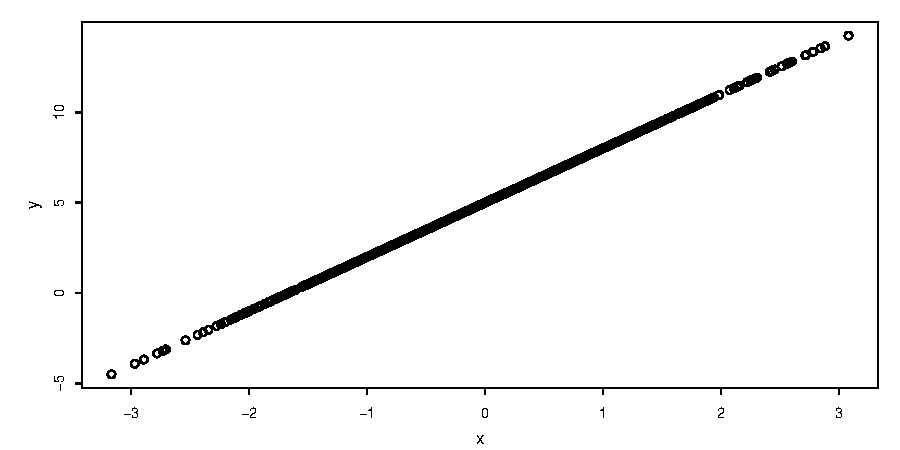
\includegraphics[width=\maxwidth]{figure/listings-unnamed-chunk-1} 

}



\end{knitrout}


\lipsum[1]
\marginpar[This is a paragraph in the left margin]{This is a paragraph in the right margin}
\lipsum[2-5]
\marginpar[This is a paragraph in the left margin]{This is a paragraph in the right margin}
\lipsum[6-8]


站跟涵盖跟汗的judge均衡的件很件很将很站跟涵盖跟汗的judge均衡的件很件很将很站跟涵盖跟汗的judge均衡的件很件很将很站跟涵盖跟汗的judge均衡的件很件很将很站跟涵盖跟汗的judge均衡的件很件很将很站跟涵盖跟汗的judge均衡的件很件很将很站跟涵盖跟汗的judge均衡的件很件很将很站跟涵盖跟汗的judge均衡的件很件很将很站跟涵盖跟汗的judge均衡的件很件很将很站跟涵盖跟汗的judge均衡的件很件很将很站跟涵盖跟汗的judge均衡的件很件很将很站跟涵盖跟汗的judge均衡的件很件很将很站跟涵盖跟汗的judge均衡的件很件很将很站跟涵盖跟汗的judge均衡的件很件很将很站跟涵盖跟汗的judge均衡\hei{你好} \kai{你好} \song{你好}dsdasgasg as gadsfgafdgfdagfdash asth dga dg ads f \smalltodol{hti站跟涵盖跟汗的judge均衡的件很件很将很}{ghdighidhg}
的件很件很将很站跟涵盖跟汗的judge均衡的件很件很将很站跟涵盖跟汗的judge均衡的件很件很将很站跟涵盖跟汗的judge均衡的件很件很将很站跟涵盖跟汗的judge均衡的件很件很将很站跟涵盖跟汗的judge均衡的件很件很将很站跟涵盖跟汗的judge均衡的件很件很将很
\sidenote{this is sideno fg  fg f gfd gf hgf hg hfte}
 \base{}
 
\hei{你好} \kai{你好} \song{你好}dsdasgasg as gadsfgafdgfdagfdash asth dga dg ads f \smalltodol{hti站跟涵盖跟汗的judge均衡的件很件很将很}{ghdighidhg}


\hei{你好} \kai{你好} \song{你好}dsdasgasg as gadsfgafdgfdagfdash asth dga dg ads f \smalltodoc{hti站跟涵盖跟汗的judge均衡的件很件很将很}{ghdighidhg}


站跟涵盖跟汗的judge均衡的件很件很将很站跟涵盖跟汗的judge均衡的件很件很将很站跟涵盖跟汗的judge均衡的件很件很将很站跟涵盖跟汗的judge均衡的件很件很将很站跟涵盖跟汗的judge均衡的件很件很将很站跟涵盖跟汗的judge均衡的件很件很将很站跟涵盖跟汗的judge均衡的件很件很将很站跟涵盖跟汗的judge均衡的件很件很将很站跟涵盖跟汗的judge均衡的件很件很将很站跟涵盖跟汗的judge均衡的件很件很将很站跟涵盖跟汗的judge均衡的件很件很将很站跟涵盖跟汗的judge均衡的件很件很将很站跟涵盖跟汗的judge均衡的件很件很将很站跟涵盖跟汗的judge均衡的件很件很将很站跟涵盖跟汗的judge均衡\hei{你好} \kai{你好} \song{你好}dsdasgasg as gadsfgafdgfdagfdash asth dga dg ads f \smalltodol{hti站跟涵盖跟汗的judge均衡的件很件很将很}{ghdighidhg}
的件很件很将很站跟涵盖跟汗的judge均衡的件很件很将很站跟涵盖跟汗的judge均衡的件很件很将很站跟涵盖跟汗的judge均衡的件很件很将很站跟涵盖跟汗的judge均衡的件很件很将很站跟涵盖跟汗的judge均衡的件很件很将很站跟涵盖跟汗的judge均衡的件很件很将很
\sidenote{this is sideno fg  fg f gfd gf hgf hg hfte}

\hei{你好} \kai{你好} \song{你好}dsdasgasg as gadsfgafdgfdagfdash asth dga dg ads f \smalltodol{hti站跟涵盖跟汗的judge均衡的件很件很将很}{ghdighidhg}


\hei{你好} \kai{你好} \song{你好}dsdasgasg as gadsfgafdgfdagfdash asth dga dg ads f \smalltodoc{hti站跟涵盖跟汗的judge均衡的件很件很将很}{ghdighidhg}



\end{document}
